\section{Collaborative filtering}
\label{sec:collab}

In this section, I discuss the first algorithmic component of the \gls{its} as depicted in Figure~\ref{fig:its-overview}, the component of exercise selection.

There are many possible factors that determine which exercise to select.
We can easily imagine some factors that are likely to have a big influence, such as the difficulty of the exercise, the vulnerability type, and the programming language.
For other factors it is more difficult to determine how important they are, or if they matter at all.
Some examples are code quality, code legibility, software type, or even just the coding style of the author of the challenge.
There are also likely other factors that we are not yet aware of.

For this reason, it is desirable to create a recommendation system that uses a black box approach.
With this kind of approach it is not necessary to know which factors determine a good recommendation.
There only need to be enough users and challenges, as well as a way to determine if a challenge was useful to a user.

One frequently used technique for recommendation systems is \gls{cf}.
In \gls{cf} a target user's affinity for items is used to find other users who are most like-minded.
This group's collective affinity for items is then used to predict the target user's affinity for those items.

These types of algorithms are most easily understood through a visual representation. 
In Figure~\ref{fig:cf} a simple example of a \gls{cf} algorithm is illustrated.
In this figure the recorded affinity of users $i$ $(i = 0,\dots,5)$ for movies $j$ $(j = A,\dots,J)$ is depicted in a two dimensional grid.
A green check mark in the grid means that the user enjoyed the movie, a red cross means they did not.
There are also many empty spaces as not all users have watched all movies.
In order to predict the affinity of a target user $i = 0$ for a target movie $j = B$, the \gls{cf} algorithm starts by finding the users who are most like-minded, the users who have the most similar recorded affinity.
For each user the algorithm determines for how many movies they have the same affinity as the target user.
In Figure~\ref{fig:cf} the affinity of the target user is marked with an orange background, affinity of other users that is the same as the target user is marked with a green background.
In the example, user $i = 1$ enjoyed movies $j \in \{A,C\}$.
But their affinity for movie $C$ is the only affinity they have in common with the target user.
Users $i \in \{2,3,5\}$ each have the same affinity as the target user for two of the movies. 
In this example they make up the group of people that are most like-minded to the target user.
To predict if the target user would enjoy the target movie $j = B$, the algorithm now uses this group's affinity for the target movie, marked in a blue background in Figure~\ref{fig:cf}.
Two of the most like-minded users enjoyed the movie and one of them did not.
Since the majority of like-minded users enjoy the target movie, the algorithm predicts the target user might enjoy it as well.

\begin{figure}
    \centering
    %\input{03-education/plots/collaborative-filtering}
    \includegraphics[page=7]{03-education/figures/tikzfigures.pdf}
    \caption[Collaborative filtering algorithm]{Visual representation of the steps to determine if the target movie $j=B$ is a good recommendation for the target user $i=0$. 
    The \gls{cf} algorithm first finds all users who have similar preferences for movies as the target user (marked in green). 
    The users who have the most similar preferences are used in a majority vote. 
    In the example users 2, 3, and 5 each had the same preference as the target user for two different movies.
    The majority of these users enjoyed the target movie (marked in blue), so the algorithm concludes that the target is a good recommendation.}
    \label{fig:cf}
\end{figure}

\subsection{Adapted to learning systems}
\label{sec:adapted-cf}
Some adjustments are needed to apply \gls{cf} to a learning system.
In a learning system a good recommendation is one that allows meaningful learning to take place and at the same time keeps the user engaged.
A good recommendation is hence based on the \textit{utility} of a user for an item, rather than their affinity.
If the users who are most like-minded increased their ability level through playing this challenge, it is likely a good recommendation.

As mentioned before, learning also has a more apparent temporal aspect to it.
An exercise that is useful to a user at the start is no longer an appropriate recommendation once their ability has increased sufficiently.
It could hence be beneficial to keep track of the ability level around which a recommendation can be deemed appropriate.
The \gls{cf} algorithm can then consider only users to be like-minded, if they experienced the same utility as the target user within a certain ability range.
Users who experienced the same utility for an item but at a sufficiently dissimilar ability level will not be considered like-minded users.

In Figure~\ref{fig:3d-cf} it is illustrated on the example algorithm from before how this adaptation could be achieved.
In this figure the recorded utility that the users $i$ $(i = 0,\dots,5)$ experienced from challenges $j$ $(j = A,\dots,J)$ is depicted in a two dimensional grid for three sufficiently distinct ability levels $\bm\theta$.
A green check mark means that this challenge was useful to the user around that ability level.
A red cross means it was not useful, and the user either did not learn anything, or the challenge caused the user to disengage from the training.
How the utility of a challenge is determined will be explained in Section~\ref{sec:utility}.
To predict the utility of the target challenge $j = B$ to the target user $i = 0$, the adapted \gls{cf} algorithm looks for the most like-minded users, the users who experienced the most similar utility.

However, only if the same utility was experienced around the same ability level does it count towards like-mindedness.
In Figure~\ref{fig:3d-cf}, utility that was experienced by the target user for challenges is marked with an orange background.
Similar utility that was experienced around the same ability level is marked with a green background.
At the lowest ability level, user $i = 2$ experienced the same utility as the target user for four challenges.
User $i = 1$, just like the target user, experienced challenge $j = C$ as useful.
However, the challenge was useful to user $i = 1$ at the lowest ability level, while the target user found this challenge useful when their ability level was sufficiently higher.
Similar utility like this that was experienced around a different ability level is marked with a red background in the figure.
This utility does not count towards like-mindedness.
Using this metric for like-mindedness, we find that users $i \in \{2,3,5\}$ each experienced the same utility around the same ability level as the target user for four different challenges.
They make up the group of users who are most like-minded to the target user.

Beyond this adaptation the same steps are used to decide the final recommendation.
The majority of like-minded users experienced the target challenge as useful around the targeted ability level, marked with a blue background.
The algorithm concludes that the target challenge is a good recommendation for the target user.

\begin{figure}
    \centering
    %\input{03-education/plots/3d-collaborative-filtering}
    \includegraphics[page=3]{03-education/figures/tikzfigures.pdf}
    \caption[Adapted collaborative filtering algorithm]{Visual representation of the steps to determine if the target challenge $j=B$ is a good recommendation for the target user $i=0$. 
    The collaborative filtering algorithm first finds all users who experienced similar utility from challenges as the target user around the same ability level $\bm\theta$ (marked in green). 
    Similar utility at a different ability level is disregarded (marked in red).
    The users who experienced the most similar utility are used in a majority vote. 
    In the example users 2, 3, and 5 each experienced the same utility as the target user for four different challenges.
    The majority of these users experienced the target challenge as useful (marked in blue), so the algorithm concludes that the target is a good recommendation.}
    \label{fig:3d-cf}
\end{figure}

\subsection{Types of collaborative filtering}
In the examples until now, the affinity (or utility) of a user for an item was considered binary, the user either liked it, or they did not.
In reality, often a more complex scale is used.
For example, Netflix movie recommendations use a rating scale between 1 and 5.
In this context, the affinity of a user $u$ for an item $i$ is often called the rating $r_{ui}$ of a user for an item.
The goal of a \gls{cf} algorithm is then to make a prediction of this rating $\hat{r}_{ui}$.
\Gls{cf} algorithms can be split into two broad categories, memory-based and model-based algorithms, based on how they set out to achieve this goal~\cite{li2021novel,sharma2017collaborative,yu2004probabilistic,breese2013empirical,su2009survey}.

\subsubsection{Memory-based}
Memory-based \gls{cf} algorithms directly use observed ratings to compute predictions.
Generally, these algorithms mark a subset of users as neighbours to the target user by calculating the similarity between users~\cite{li2021novel,Hug2020}.
They then use the neighbour's ratings to predict the rating of the target user~\cite{su2009survey,Hug2020,Koren2010,Ricci2010}.

Memory-based \gls{cf} algorithms are frequently used in recommender systems and even commercial systems such as the Amazon webstore~\cite{sharma2017collaborative,yu2004probabilistic}.
The main advantages of memory-based collaborative filtering algorithms are that they are easy to implement, and that new data can be added easily and incrementally.
Their biggest shortcoming is a decreased performance for sparse data, when it is difficult to find sufficient neighbours.
They also can not make recommendations for new users or items as there is no data to do similarity computations with.
In the \gls{its} however, we already need sufficient data to compute the difficulty and ability estimates.
In a learning system the need for an initial calibration phase can not be avoided, so this shortcoming does not impact the design of the \gls{its}.

Five different memory-based \gls{cf} algorithms are considered in this work. 
They will be described in more detail in the experiments in Section~\ref{sec:eval-cf}.
Four of these algorithms are \gls{knn} algorithms, they first determine the k nearest neighbours and use the ratings of these neighbours to compute a prediction.
Because these algorithms use a very explicit definition of similarity between users, they can be easily adapted to learning systems by changing this definition to take into account the ability of the users.
The remaining memory-based algorithm uses the ratings of all users to make a prediction, adapting it to learning systems will be harder, but can still be achieved by processing the data, as will be explained in the description of the experiments.

\subsubsection{Model-based}
Model-based \gls{cf} algorithms use statistical and machine learning methods to construct a model, and use this model to make predictions~\cite{sharma2017collaborative, li2021novel,sarwar2002recommender,heckerman2000dependency}.
These models often use techniques to reduce the dimensions of the matrix of user-item ratings.
This reduces the scalability and sparsity problems that are experienced by memory-based algorithms~\cite{sarwar2002recommender,moreno2016web}.
Model-based algorithms are often more accurate, but the construction of the model is often slow and expensive, and they have to be re-built when new data is being added incrementally.

Algorithms using clustering techniques are simple examples of model-based algorithms~\cite{su2009survey,breese2013empirical,sarwar2002recommender,o1999clustering}.
Users or items are assigned to one or more clusters so that the matrix of user-item ratings becomes a smaller, denser matrix of clusters.
It is then possible to use statistics from these clusters to make predictions, for example, by taking the average rating of a cluster.
In the experiments of this work, one clustering algorithm is evaluated.

Thanks to their accuracy and scalability, model-based algorithms based on matrix factorization have gained a lot in popularity~\cite{Ricci2010}.
These algorithms, use the technique of \gls{svd}, to make a low rank approximation of the original ratings matrix~\cite{george2005scalable, Ricci2010, Hug2020}.
\Gls{svd} is a well established technique in linear algebra and machine learning to identify latent semantic factors.
Applying it in the \gls{cf} domain raises a few difficulties due to the sparsity of the rating matrix, which increases the risk of overfitting.

In the experiments of this work, I evaluated \gls{pmf}~\cite{mnih2008probabilistic}, \gls{nnmf}~\cite{wang2012nonnegative,hoyer2004non}, \gls{svd}~\cite{sarwar2000application,polat2005svd,Ricci2010}, and \gls{svd}++~\cite{koren2008factorization,Ricci2010}.
All of these algorithms are explained in more detail in Section~\ref{sec:eval-cf}.

\subsection{Alternative approaches}
\label{sec:cf-alternatives}

\paragraph{Adaptive learning systems}
Many computerized learning systems already exist, both in commercial offerings and in research literature.
Older systems do not consider individual learners needs, but made decisions based on pre-planned instructions for the field of study.
As a result, these systems do not provide individual attention to students as a natural (human) teacher would~\cite{mahdi2016intelligent}.
This inspired the rise of more advanced learning systems that consider both the field and the learner to provide flexibility in the presentation of the educational material.
Some such systems have been built to teach computer science concepts, such as debugging~\cite{carter2013tutoring}, cryptographic algorithms~\cite{abuel2018intelligent,mahdi2016intelligent}, programming in C++~\cite{abu2009evaluating}.

Existing systems have varying degrees of intelligence and adaptiveness.
In commercial offerings, such as Pluralsight Iris\footnote{\url{https://www.pluralsight.com/product/iris}}, adaptive learning often refers to an initial calibration phase to determine the initial ability level of a user.
In other systems, students are allowed to advance to more difficult levels when a sufficiently high accuracy is achieved on exercises in the current level~\cite{abu2009evaluating,mahdi2016intelligent}.
Some more advanced systems provide adaptive feedback to the users, based on which mistakes have been made in the exercises~\cite{carter2013tutoring,abuel2018intelligent}.
Finally, the most advanced systems are able to adapt the difficulty of the exercises more dynamically.
Duolingo for example, adapts the difficulty of the of last few exercises in a lesson based on the performance of the student on the previous exercises\footnote{\url{https://blog.duolingo.com/keeping-you-at-the-frontier-of-learning-with-adaptive-lessons/}}.

All of these system focus on offering exercises of the appropriate difficulty level.
The goal of the \gls{its} is to also pay attention to other potential factors influencing usability, engagement and hence learning.

\paragraph{Computerized Adaptive Tests}
\Glspl{cat} are computer-based tests that adapt to the ability of the examinee. 
They continuously estimate the ability level and serve the next test item based on the current estimate.
While there are techniques from \glspl{cat} that are useful to us, as will be explained in Section~\ref{sec:calib}, the item selection is not appropriate for use in the \gls{its}.

This is because the goal of a test is to estimate the ability of an examinee. \Glspl{cat} are able to maintain a higher precision of ability estimation while being about 50\% shorter compared to \glspl{fit}~\cite{weiss1984application}.
To estimate the examinee's ability in such an efficient way, \glspl{cat} select the next item in a test based on which one provides the most information about the examinee. 
These are the items for which the probability of a correct answer is around 50\%~\cite{magis2017computerized, ling2017computerized}.

This goal is of course different from that of the \gls{its} which is to motivate and engage the users. 
In fact, the opposite is even true, tests are inherently not very motivating.
Certainly that is the case for \glspl{cat}, where the examinee is only expected to correctly answer half of the test questions.
Research has shown that engagement can be improved, and anxiety reduced, by choosing items for which the probability of a correct answer is higher (e.g. 70\%)~\cite{ling2017computerized}. 
Still, the item selection algorithm in \glspl{cat} only takes into account the difficulty of the items. 
As discussed before, we want the \gls{its} to possibly take into account other aspects of the exercises, such as coding style, author, or application type.